% Chapitre 7 : La Gestion des Projets Logiciels

\section{Chapitre 7 : La Gestion des Projets Logiciels}



La gestion des projets logiciels vise à structurer méthodiquement et progressivement une réalité à venir, en appliquant un objectif et des actions à entreprendre avec des ressources données. Le rôle du chef de projet est de planifier, organiser et contrôler l'ensemble des activités nécessaires à la réalisation du projet.



\subsection{Organisation du Projet (WBS, PBS, OBS)}



Trois outils structurants ont guidé l'organisation du projet.



Le \textbf{Work Breakdown Structure (WBS)} décompose le projet en tâches hiérarchiques. Pour SaaS Directory, le WBS s'articule autour de cinq phases principales (fondations, profil, marketplace, messagerie, monétisation), chacune subdivisée en tâches techniques (développement frontend, développement backend, tests, documentation).



Le \textbf{Product Breakdown Structure (PBS)} identifie les livrables de chaque phase : authentification fonctionnelle, profil utilisateur opérationnel, produit lancable sur le marketplace, système de messagerie temps réel, et système d'abonnements Free/Pro.



Le \textbf{Organizational Breakdown Structure (OBS)} répartit les responsabilités. Le projet a été réalisé par deux développeurs en binôme, avec une répartition naturelle des tâches selon les compétences (frontend React vs backend Server Actions).



\subsection{Planification (GANTT, PERT)}



La planification du projet a utilisé un diagramme de GANTT pour visualiser les cinq phases sur une échelle temporelle. Chaque phase correspond à un sprint de développement d'environ trois à quatre semaines, avec des jalons intermédiaires (MVP marketplace, messagerie fonctionnelle).



\begin{figure}[H]

\centering

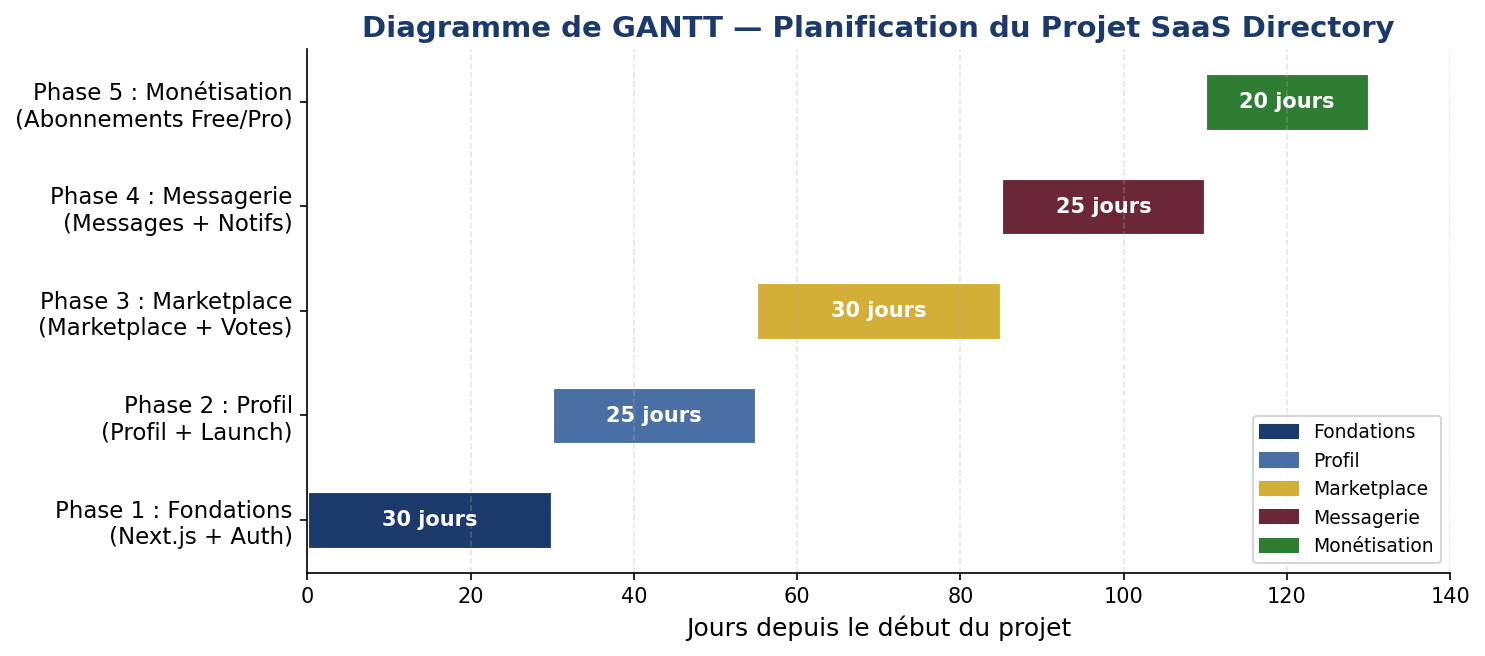
\includegraphics[width=0.95\textwidth]{assets/gantt.png}

\caption{Diagramme de GANTT — Planification du Projet SaaS Directory}

\label{fig:gantt}

\end{figure}



La figure~\ref{fig:gantt} présente la répartition temporelle des cinq phases du projet sur une échelle de 130 jours. La Phase 1 (Fondations) occupe les 30 premiers jours, suivie par le Profil (25 jours), le Marketplace (30 jours), la Messagerie (25 jours), et enfin la Monétisation (20 jours).



Le diagramme PERT (Program Evaluation and Review Technique) modélise les dépendances entre tâches. Les liaisons principales sont de type "fin à début" : l'authentification (Phase 1) doit être terminée avant le profil (Phase 2) ; le profil avant le marketplace (Phase 3) ; le marketplace avant la messagerie (Phase 4) ; la messagerie avant la monétisation (Phase 5).



\subsection{Estimation des Coûts par COCOMO}



L'estimation des coûts d'un projet logiciel est un exercice délicat. Les raisons classiques de dépassement incluent l'optimisme, la négligence des problèmes techniques, le manque d'expérience, l'oubli de la documentation, et la sous-estimation des tâches annexes. Pour contrer ces biais, nous avons appliqué la méthode COCOMO (COnstructive COst MOdel) de Barry Boehm, un modèle d'estimation empirique basé sur la taille du projet en KLOC.



\subsubsection{Taille du Projet}



Le codebase de SaaS Directory compte 12 166 lignes de code réparties sur 108 fichiers TypeScript/TSX, soit approximativement 14 KLOC. Cette taille inclut le code source applicatif (\texttt{src/app} : 3 198 LOC, \texttt{src/components} : 5 234 LOC, \texttt{src/lib} : 2 957 LOC), les tests (\texttt{src/test} : 111 LOC, \texttt{e2e} : 33 LOC), et les scripts (1 115 LOC).



\subsubsection{Application du COCOMO de Base}



Pour un projet web moderne avec une stack technologique récente (Next.js 16.2.4, React 19.2.4, TypeScript 5), nous avons retenu le mode semi-détaché (projet moyennement complexe, équipe avec expérience mixte, contraintes modérées). Les coefficients du mode semi-détaché sont $a = 3{,}0$ et $b = 1{,}12$.



\begin{table}[H]

\centering

\caption{Estimation COCOMO de Base — Mode Semi-Détaché (14 KLOC)}

\label{tab:cocomo}

\begin{tabular}{@{}lll@{}}

\toprule

\textbf{Paramètre} & \textbf{Formule / Valeur} & \textbf{Résultat} \\

\midrule

Taille du projet & 12 166 LOC $\approx$ 14 KLOC & 14 KLOC \\

Mode de développement & Semi-Détaché & $a = 3{,}0$ ; $b = 1{,}12$ \\

Effort estimé & $E = a \times (\text{KLOC})^b$ & $E \approx 58$ Personnes-Mois \\

Durée estimée & $D = 2{,}5 \times E^{0{,}35}$ & $D \approx 9{,}5$ mois \\

Taille d'équipe théorique & $N = E / D$ & $N \approx 6$ personnes \\

\midrule

\textbf{Taille d'équipe réelle} & \textbf{2 développeurs sur 5 mois} & \textbf{10 Personnes-Mois} \\

\bottomrule

\end{tabular}

\end{table}



Ces chiffres constituent une estimation théorique à visée pédagogique. En réalité, le projet a été réalisé par deux développeurs travaillant en parallèle sur une période académique d'environ cinq mois, soit environ 10 Personnes-Mois. Cet écart illustre la différence fréquente entre les modèles prédictifs et la réalité des projets académiques en mode agile.

